\section{Background}

\begin{frame}{Evolutionary Algorithm: Example}
\begin{figure}
  \includemedia[width=\linewidth,height=0.6\textwidth, flashvars={scaleMode=zoom}]{}{http://www.youtube.com/v/z9ptOeByLA4?t=1m08s&amp;rel=0&amp;showinfo=0}
  \captionsetup{singlelinecheck=off,justification=raggedright}
\href{https://youtu.be/z9ptOeByLA4?t=1m08s}{\caption{Evolution in Action \cite{Cheney2013UnshacklingEncoding}}}
\end{figure}
\end{frame}

\begin{frame}{Evolutionary Algorithm: Problem Statement}
  
  \begin{columns}
\begin{column}{0.6\textwidth}
 What makes an evolutionary algorithm work?
\end{column}
\begin{column}{0.4\textwidth}
\begin{center}
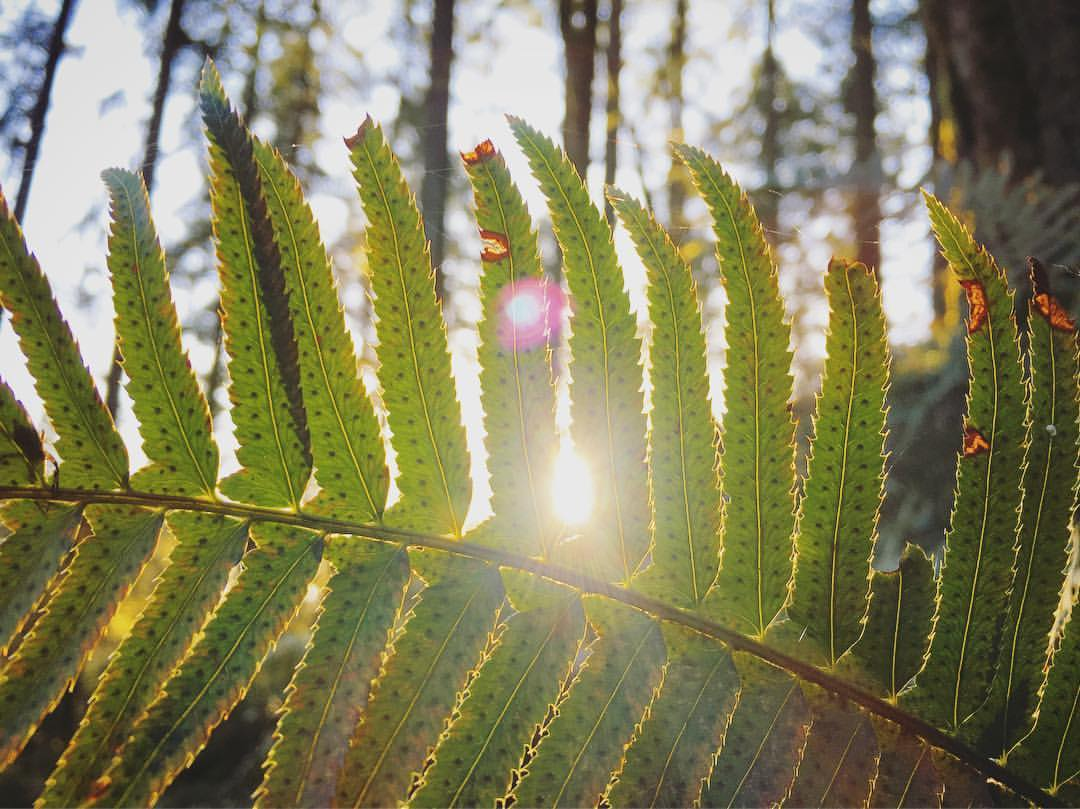
\includegraphics[width=\textwidth,trim={7cm 0 13cm 0},clip]{img/sunfern}
\end{center}
\end{column}
\end{columns}
\end{frame}

\begin{frame}{Defining Evolvability}
consensus: the amount of \textcolor{h2}{viable} \textcolor{h1}{variation} generated by the evolutionary process
\begin{itemize}
  \item evolvability as the amount of \textcolor{h1}{\textbf{novel variation}} generated
  \item evolvability the proportion of variation that is \textcolor{h2}{\textbf{viable}}
\end{itemize}
\end{frame}

% \begin{frame}{The Evolvability Conundrum}
% How can natural selection ``favor properties hat may prove useful to a given lineage in the future, but have no present adaptive function''? \cite{Pigliucci2008IsEvolvable}
% \end{frame}


\subsection{Evolvability as Novel Variation}

\begin{frame}{Evolvability as Novel Variation}
	\begin{figure}
 \centering
    \begin{subfigure}[b]{0.5\textwidth}
        \centering
    	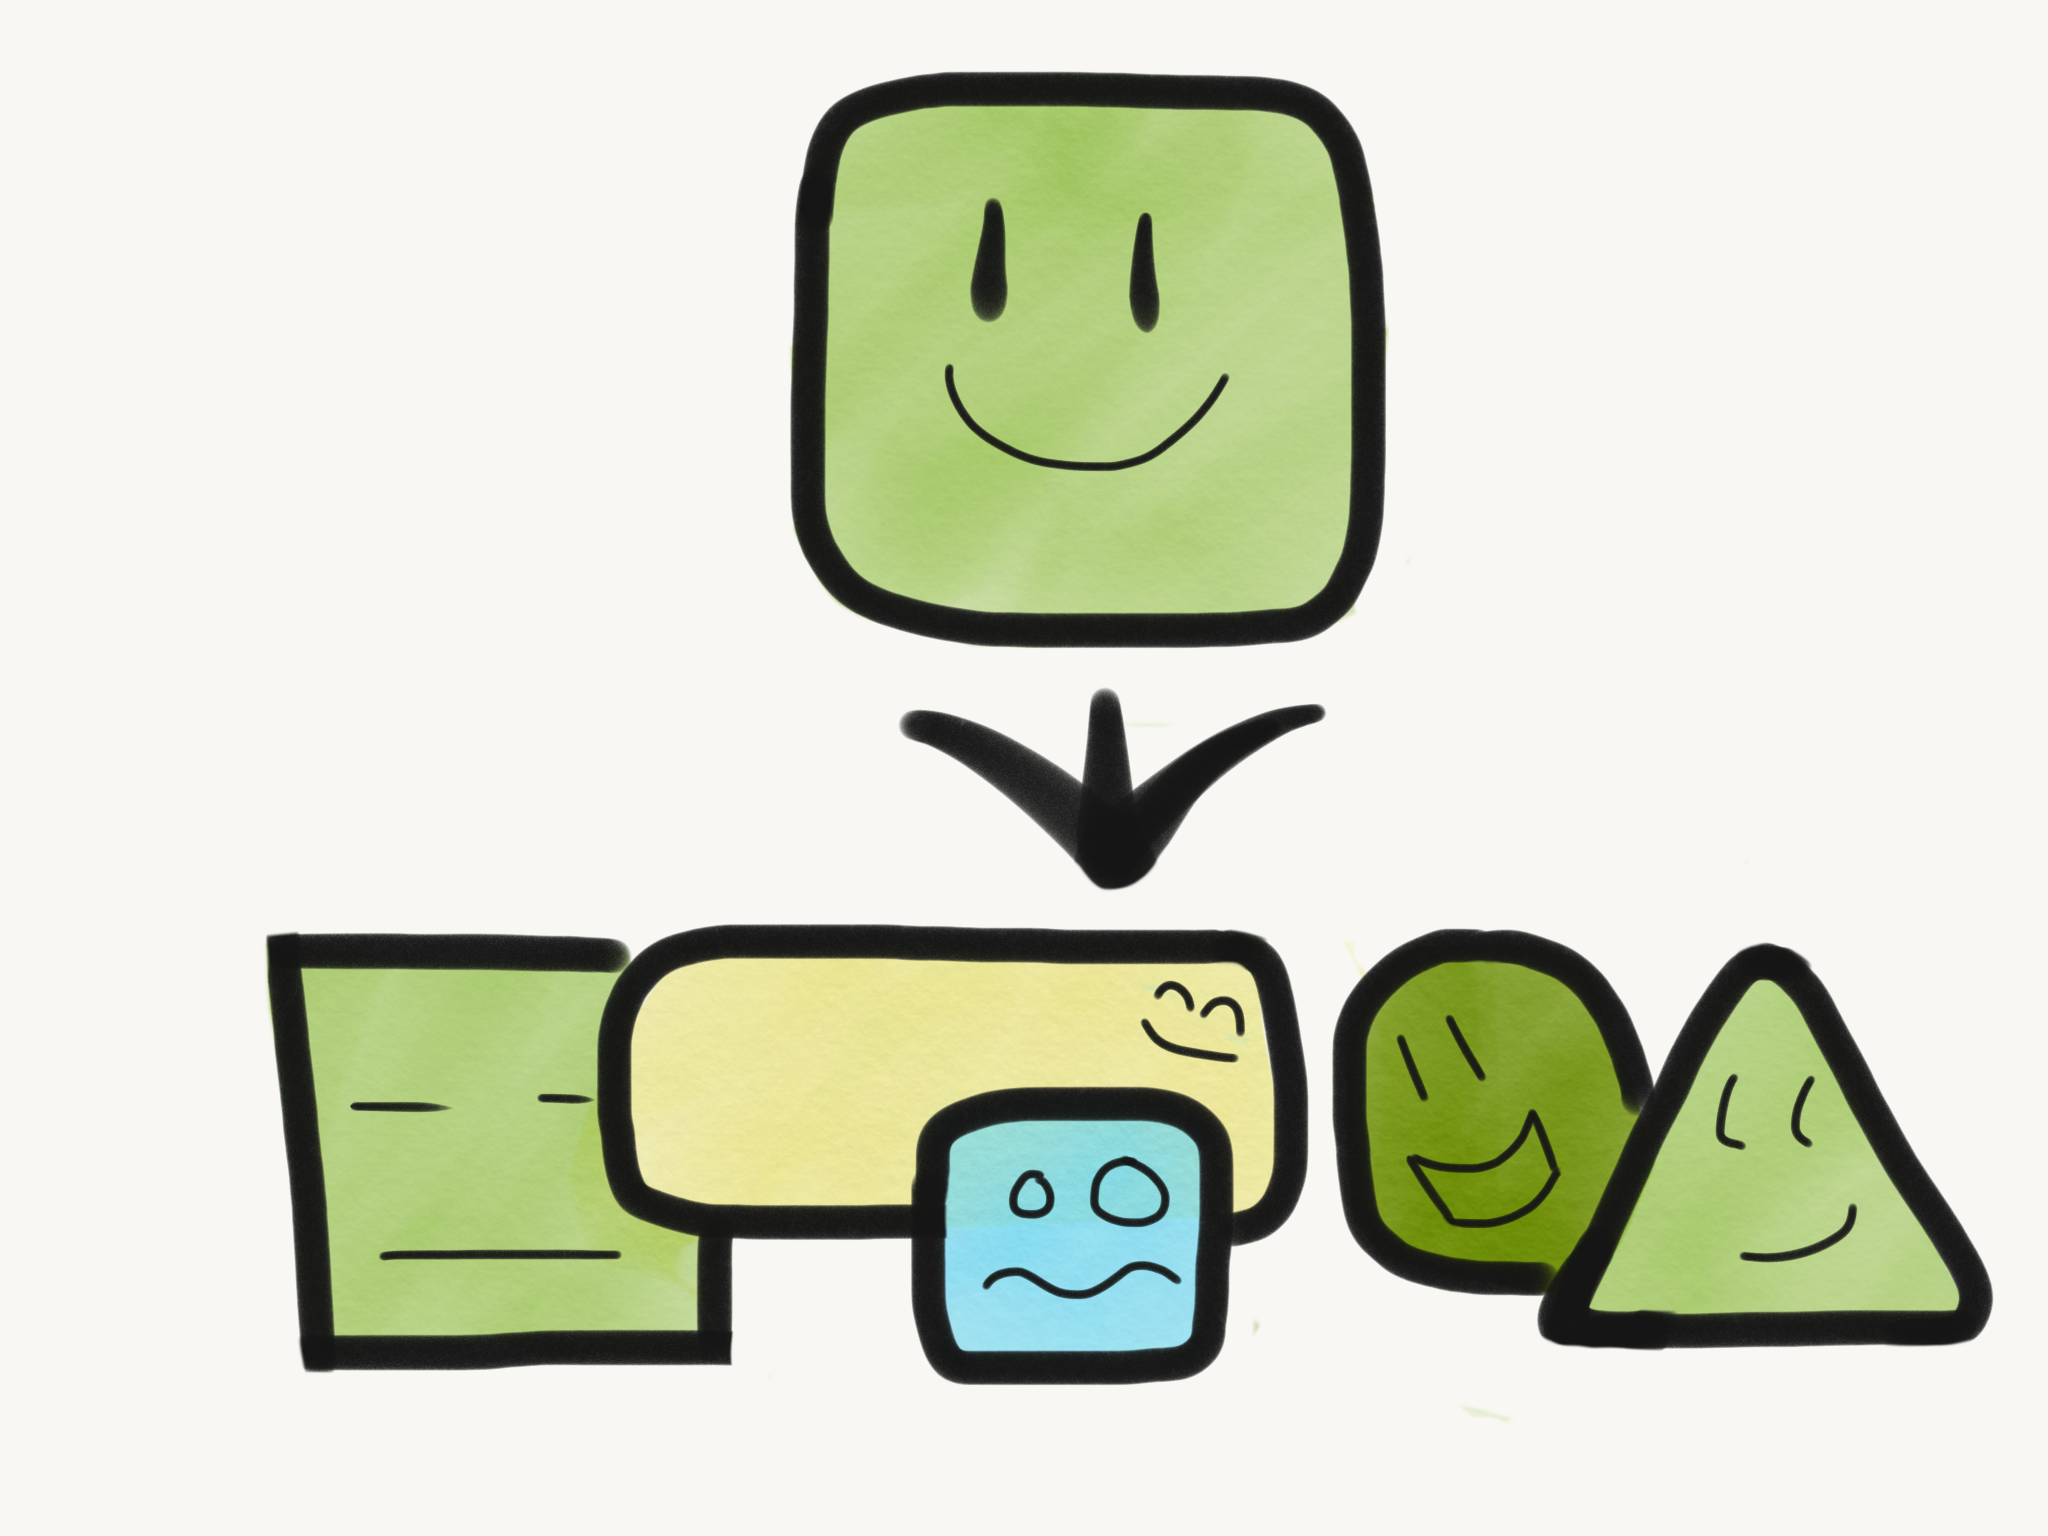
\includegraphics[width=\textwidth]{img/individual_evolvability.png}
        \caption{high individual evolvability}
        \label{subfig:canalization}
    \end{subfigure}%
    \hfill
    \begin{subfigure}[b]{0.5\textwidth}
        \centering
        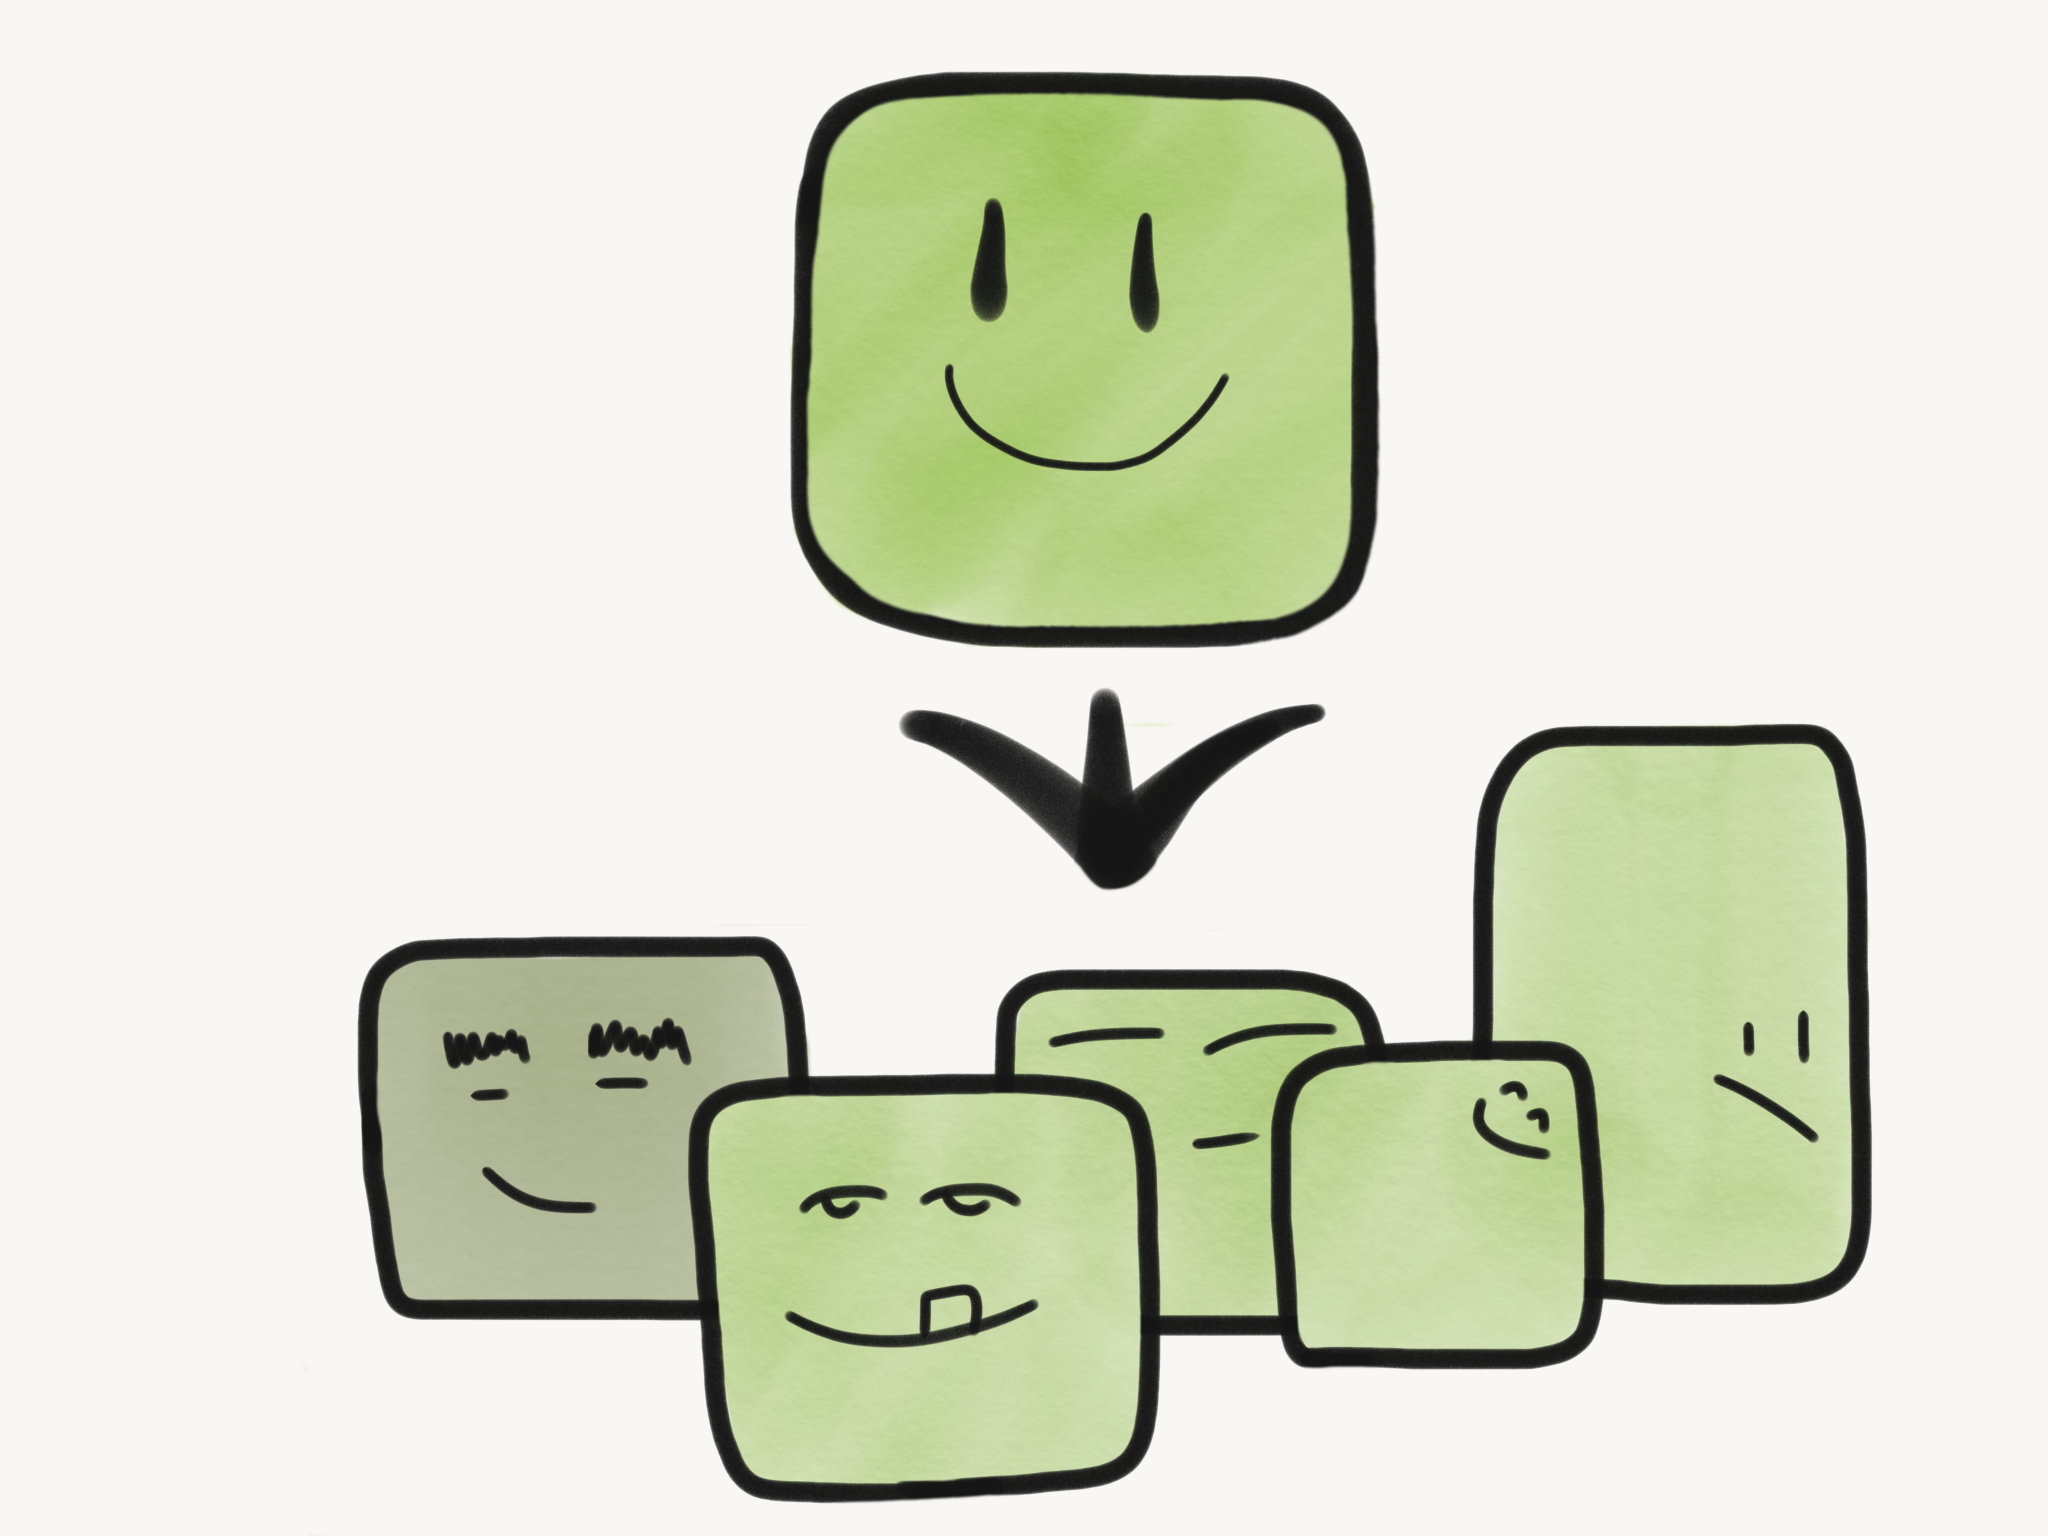
\includegraphics[width=\textwidth]{img/low_individual_evolvability.png}
        \caption{low individual evolvability}
        \label{subfig:no_canalization}
    \end{subfigure}
 	\captionsetup{singlelinecheck=off,justification=raggedright}
    \vspace{-4ex}
  \captionsetup{singlelinecheck=off,justification=raggedright}
  \caption{An illustration of individual evolvability, considering evolvability as heritable variation \cite{Wilder2015ReconcilingEvolvability}.}
  \label{fig:high_vs_low_individual_evolvability}
\end{figure}
\end{frame}

\subsection{Evolvability as Bias towards Viable Variation}

\begin{frame}{Evolvability as Bias towards Viable Variation}
  \begin{figure}
    \centering
    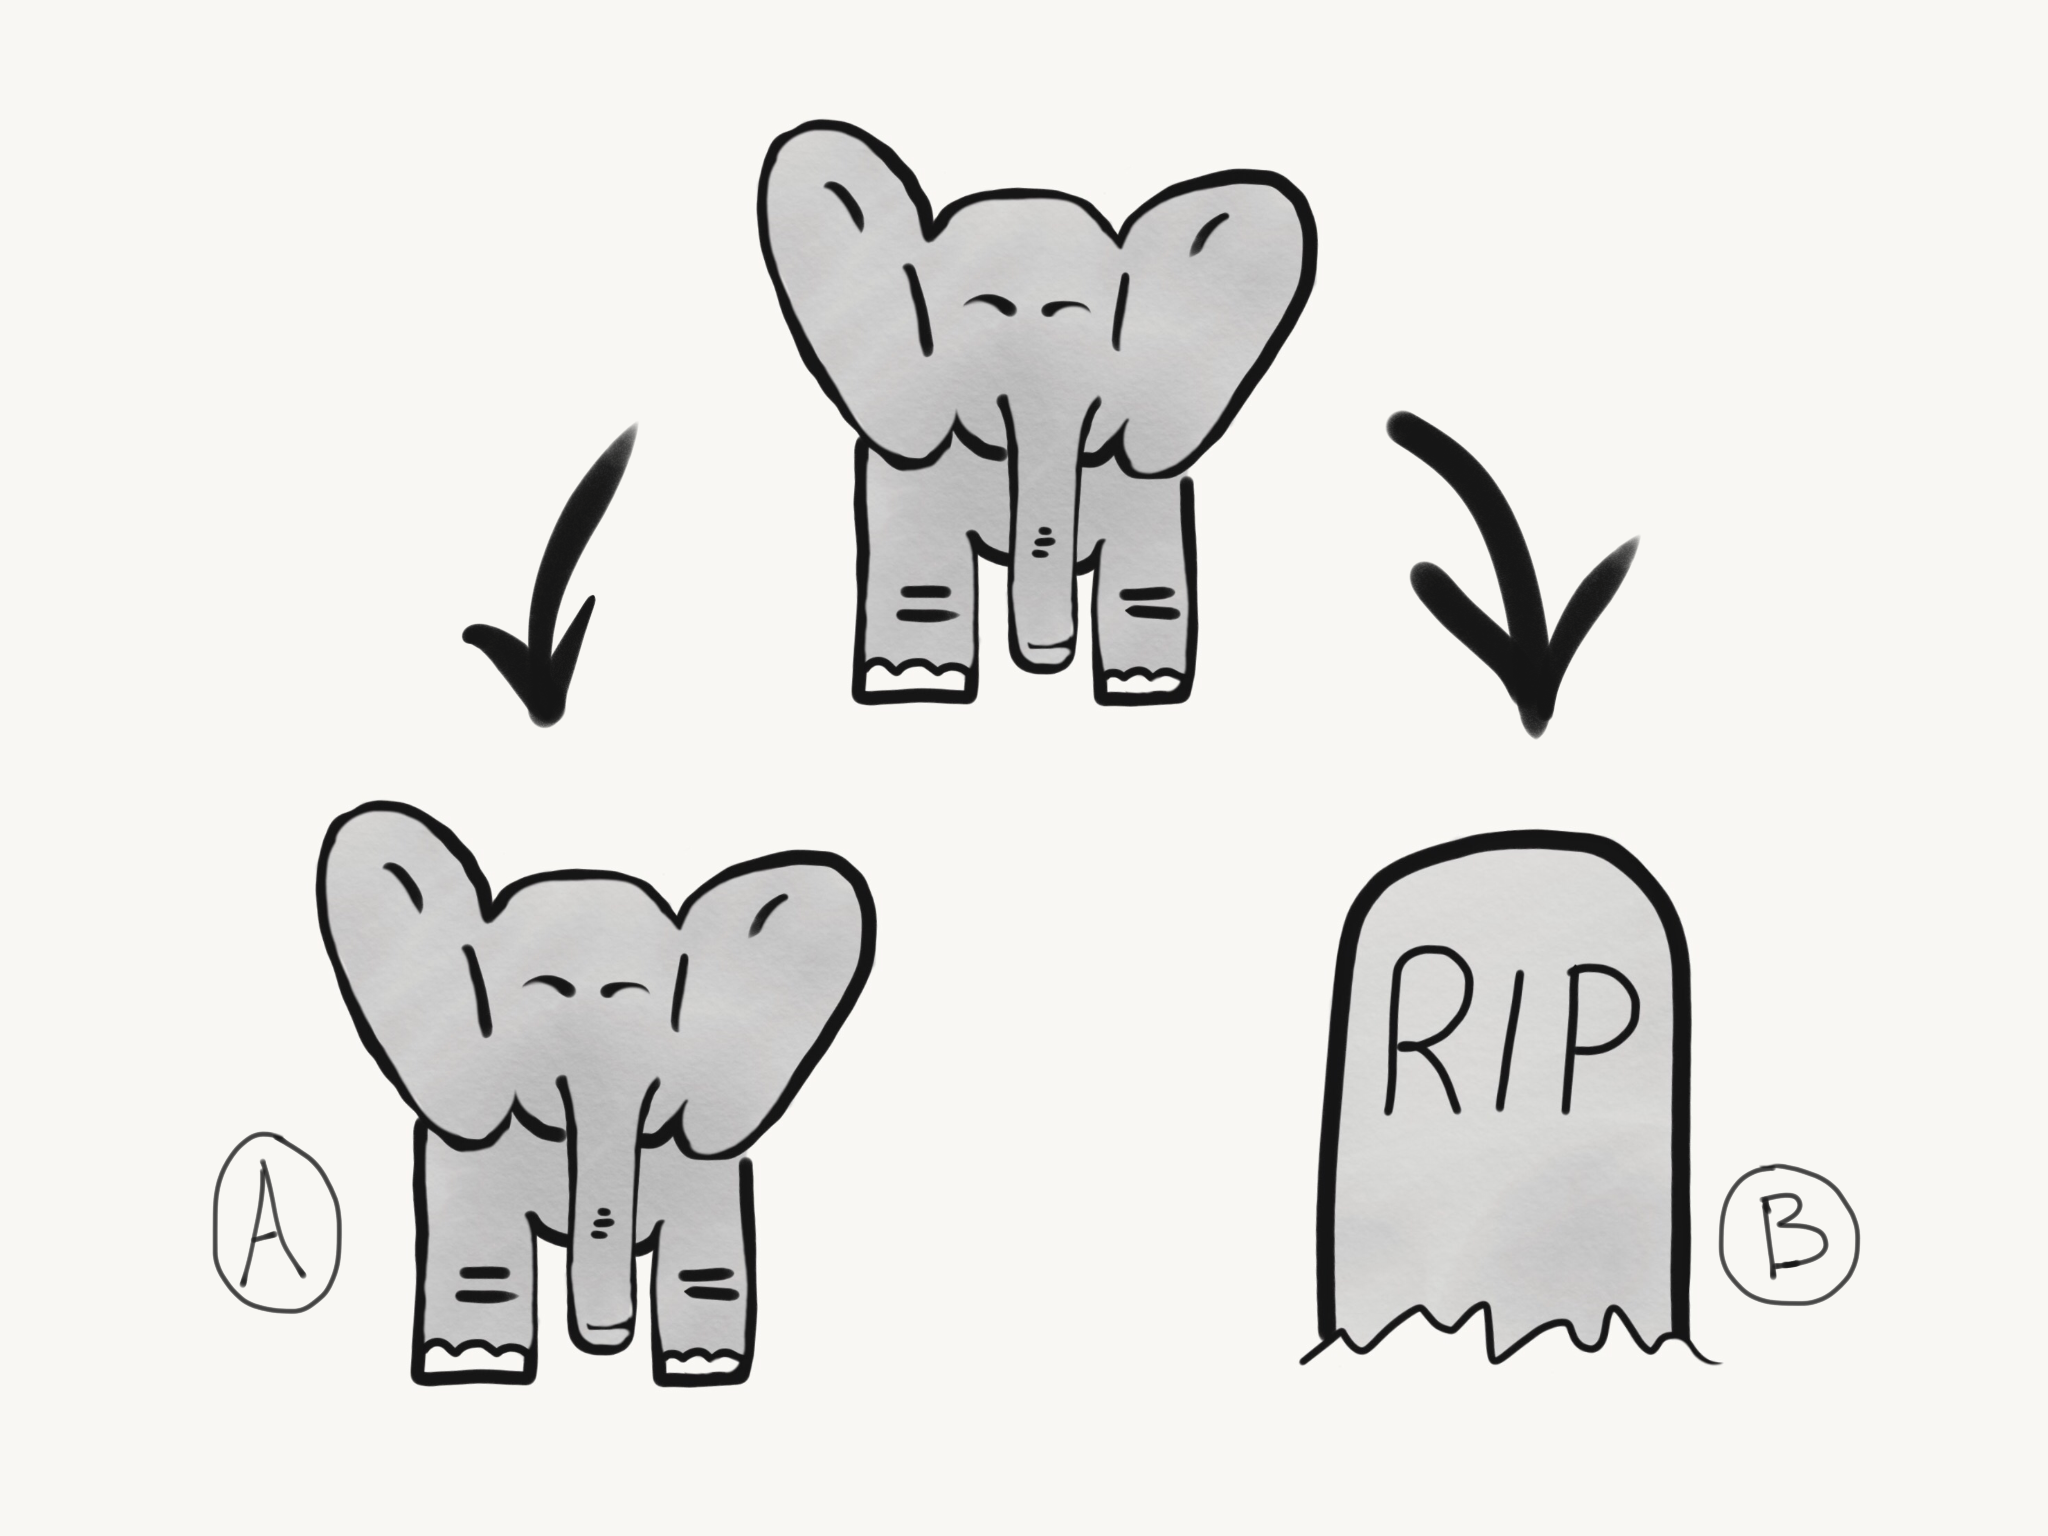
\includegraphics[width=0.8\textwidth]{img/robustness}
 	\captionsetup{singlelinecheck=off,justification=raggedright}
  	\caption{Illustration of robustness; high evolvability left and low evolvability right \cite{Downing2015IntelligenceSystems}.}
    \label{fig:robustness}
\end{figure}
\end{frame}

